\chapter{カレントミラーを組み合わせた折り返し型アナログ乗算回路}

    \section{回路構成}
        序論で述べたS/N比向上のための方針として,折り返しカスコードの構成をとることが考えられる.図\ref{fig:3_folded_gilbert}に折り返しカスコード型の乗算回路を示す.
        \begin{figure}[!b]
            \begin{center}
                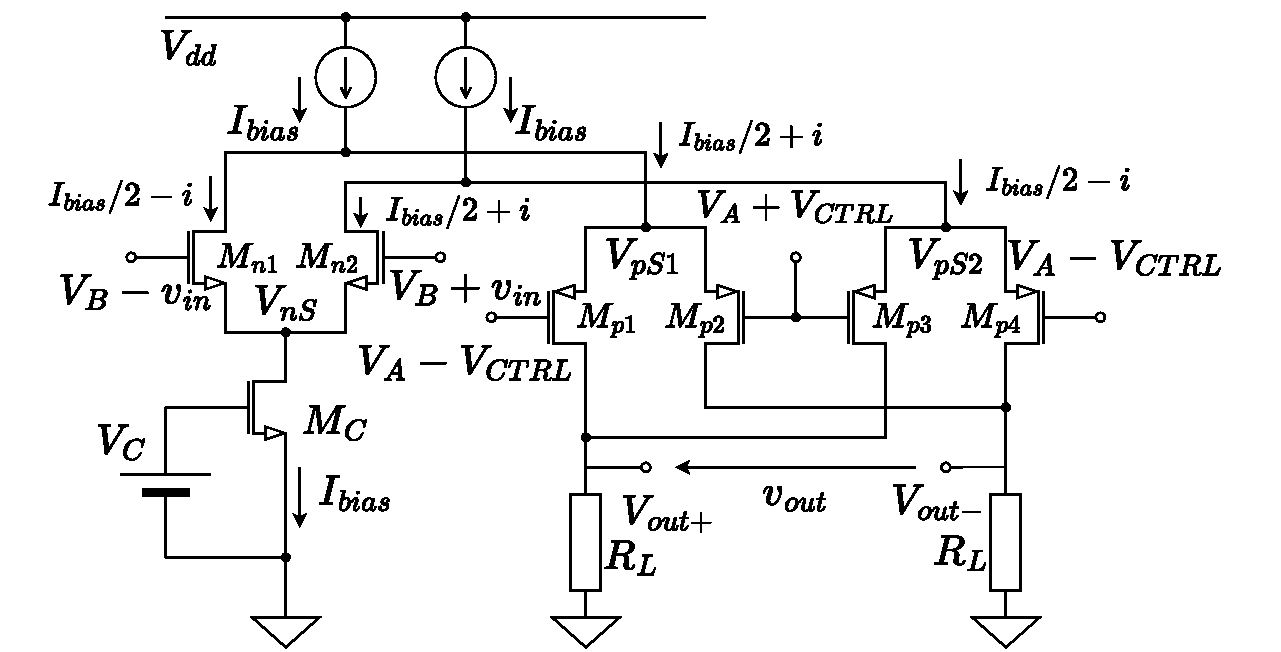
\includegraphics[width=0.99\linewidth]{figures/chapter3/folded_gilbert.pdf}
                \caption{折り返しカスコード型乗算回路}
                \label{fig:3_folded_gilbert}
            \end{center}
        \end{figure}
        この構造では定電流源を用いることで各入力の差動対$\mathrm{M_{B}}$に流れる信号電流の増減が$\mathrm{M_{p}}$に反転して伝えられる.ゲート接地増幅回路としてはpMOSFET($\mathrm{M_{p1}}$~$\mathrm{M_{p4}}$)を用いることで制御電圧に比例したトランスコンダクタンスを得る.このような折り返しカスコード型の構造をとることで出力電圧は$M_{p}$と電流源のPMOSFETで分圧するため,入力電圧分出力振幅が広がることが予測される.しかし左右それぞれにバイアス電流を流すため消費電流が増加する.また,電流源に用いるPMOSFETが十分な電流を供給できないこと,そしてPMOSFETを小信号に使用するためどうしてもNMOSFETのみのギルバート乗算回路よりも遮断周波数が低下するといったデメリットが考えられる.まずはPMOSFETの代わりに理想的な電流源を用いて$\mathrm{RHOM\;0.18\mu\;m\;Process}$にてギルバート乗算回路と折り返しカスコード型の乗算回路をバイアス電流が同じになるように設計したときのそれぞれの素子値を表\ref{table:3_gilbert_param},表\ref{table:3_folded_gilbert_param}に示す.またこの素子値におけるシミュレーションでの周波数特性を図\ref{fig:3_gilbert_ac},図\ref{fig:3_folded_gilbert_ac}にそれぞれ示す.
        \begin{table}[!b]
            \begin{minipage}[t]{.45\textwidth}
                \begin{center}
                    \caption{比較用に設計したギルバート乗算回路}
                    \label{table:3_gilbert_param}
                    \begin{tabular}{c|c|r}
                        \hline
                        \multicolumn{2}{c}{Gilbert}   & \multicolumn{1}{c}{Value}     \\
                        \hline\hline
                        &   Channel Length   &   0.72 $\mathrm{\mu m}$   \\
                        \cline{2-3}
                        $\mathrm{M_{A}}$   &   Channel Width   &   4.27 $\mathrm{\mu m}$   \\
                        \cline{2-3}
                            &   Multifinger   & 10    \\
                        \hline
                        &   Channel Length   &   0.72 $\mathrm{\mu m}$   \\
                        \cline{2-3}
                        $\mathrm{M_{B}}$   &   Channel Width   &   4.27 $\mathrm{\mu m}$   \\
                        \cline{2-3}
                            &   Multifinger   & 20    \\
                        \hline
                        &   Channel Length   &   0.72 $\mathrm{\mu m}$   \\
                        \cline{2-3}
                        $\mathrm{M_{C}}$   &   Channel Width   &   11.6 $\mathrm{\mu m}$   \\
                        \cline{2-3}
                            &   Multifinger   & 40    \\
                        \hline
                        \multicolumn{2}{c|}{$\mathrm{V_{dd}}$} &   1.8 $\mathrm{V}$   \\
                        \hline
                        \multicolumn{2}{c|}{$\mathrm{V_{A}}$} &   1.59 $\mathrm{V}$   \\
                        \hline
                        \multicolumn{2}{c|}{$\mathrm{V_{B}}$} &   1.09 $\mathrm{V}$   \\
                        \hline
                        \multicolumn{2}{c|}{$\mathrm{V_{C}}$} &   0.65 $\mathrm{V}$   \\
                        \hline
                        \multicolumn{2}{c|}{$\mathrm{R_{L}}$} &   300 $\mathrm{\Omega}$   \\
                        \hline
                    \end{tabular}
                \end{center}                
            \end{minipage}
            %
            \hfill
            %
            \begin{minipage}[t]{.45\textwidth}
                \begin{center}
                    \caption{設計した折り返しカスコード型乗算回路}
                    \label{table:3_folded_gilbert_param}
                    \begin{tabular}{c|c|r}
                            \hline
                            \multicolumn{2}{c}{Folded Cascode}   & \multicolumn{1}{c}{Value}     \\
                            \hline\hline
                            &   Channel Length   &   0.72 $\mathrm{\mu m}$   \\
                            \cline{2-3}
                            $\mathrm{M_{p}}$   &   Channel Width   &   20 $\mathrm{\mu m}$   \\
                            \cline{2-3}
                                &   Multifinger   & 10    \\
                            \hline
                            &   Channel Length   &   0.72 $\mathrm{\mu m}$   \\
                            \cline{2-3}
                            $\mathrm{M_{B}}$   &   Channel Width   &   4.27 $\mathrm{\mu m}$   \\
                            \cline{2-3}
                                &   Multifinger   & 20    \\
                            \hline
                            &   Channel Length   &   0.72 $\mathrm{\mu m}$   \\
                            \cline{2-3}
                            $\mathrm{M_{C}}$   &   Channel Width   &   11.6 $\mathrm{\mu m}$   \\
                            \cline{2-3}
                                &   Multifinger   & 40    \\
                            \hline
                            \multicolumn{2}{c|}{$\mathrm{V_{dd}}$} &   1.8 $\mathrm{V}$   \\
                            \hline
                            \multicolumn{2}{c|}{$\mathrm{V_{A}}$} &   1.59 $\mathrm{V}$   \\
                            \hline
                            \multicolumn{2}{c|}{$\mathrm{V_{B}}$} &   1.09 $\mathrm{V}$   \\
                            \hline
                            \multicolumn{2}{c|}{$\mathrm{V_{C}}$} &   0.65 $\mathrm{V}$   \\
                            \hline
                            \multicolumn{2}{c|}{$\mathrm{R_{L}}$} &   300 $\mathrm{\Omega}$   \\
                            \hline
                    \end{tabular}
                \end{center}
            \end{minipage}
        \end{table}
        \begin{figure}[!b]
            \centering
            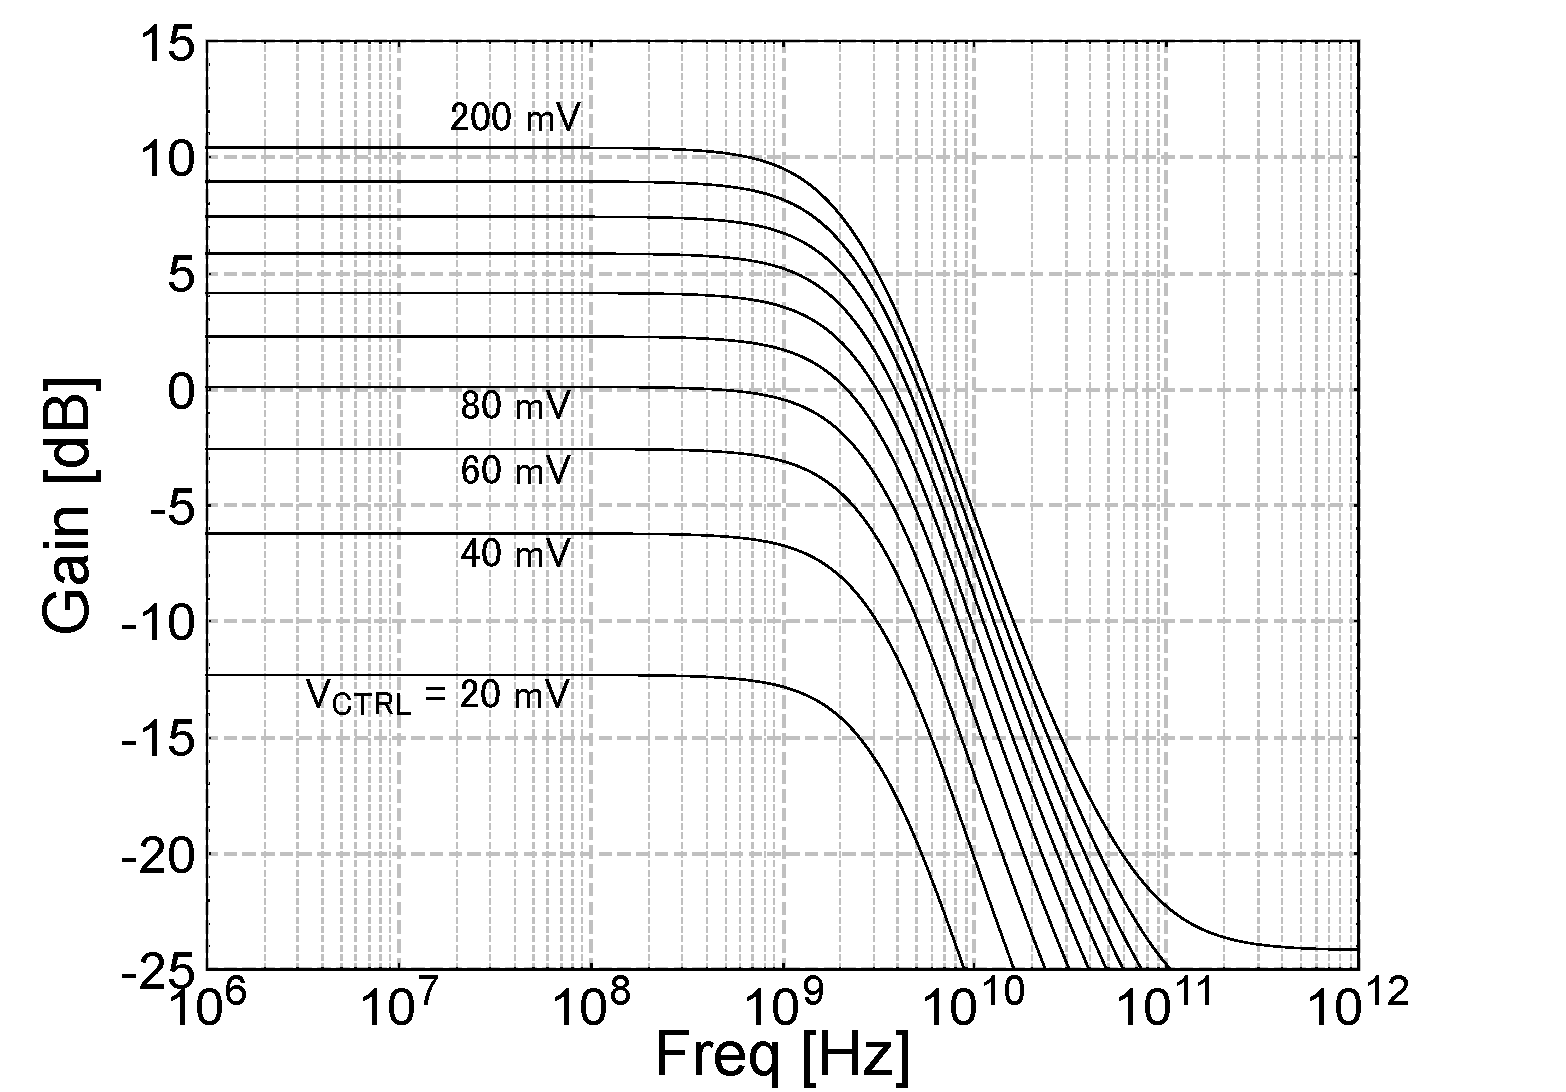
\includegraphics[width=0.99\textwidth]{figures/chapter3/previous_ac.pdf}
            \caption{ギルバート乗算回路の周波数特性}
            \label{fig:3_gilbert_ac}
        \end{figure}
        \begin{figure}[!b]
            \centering
            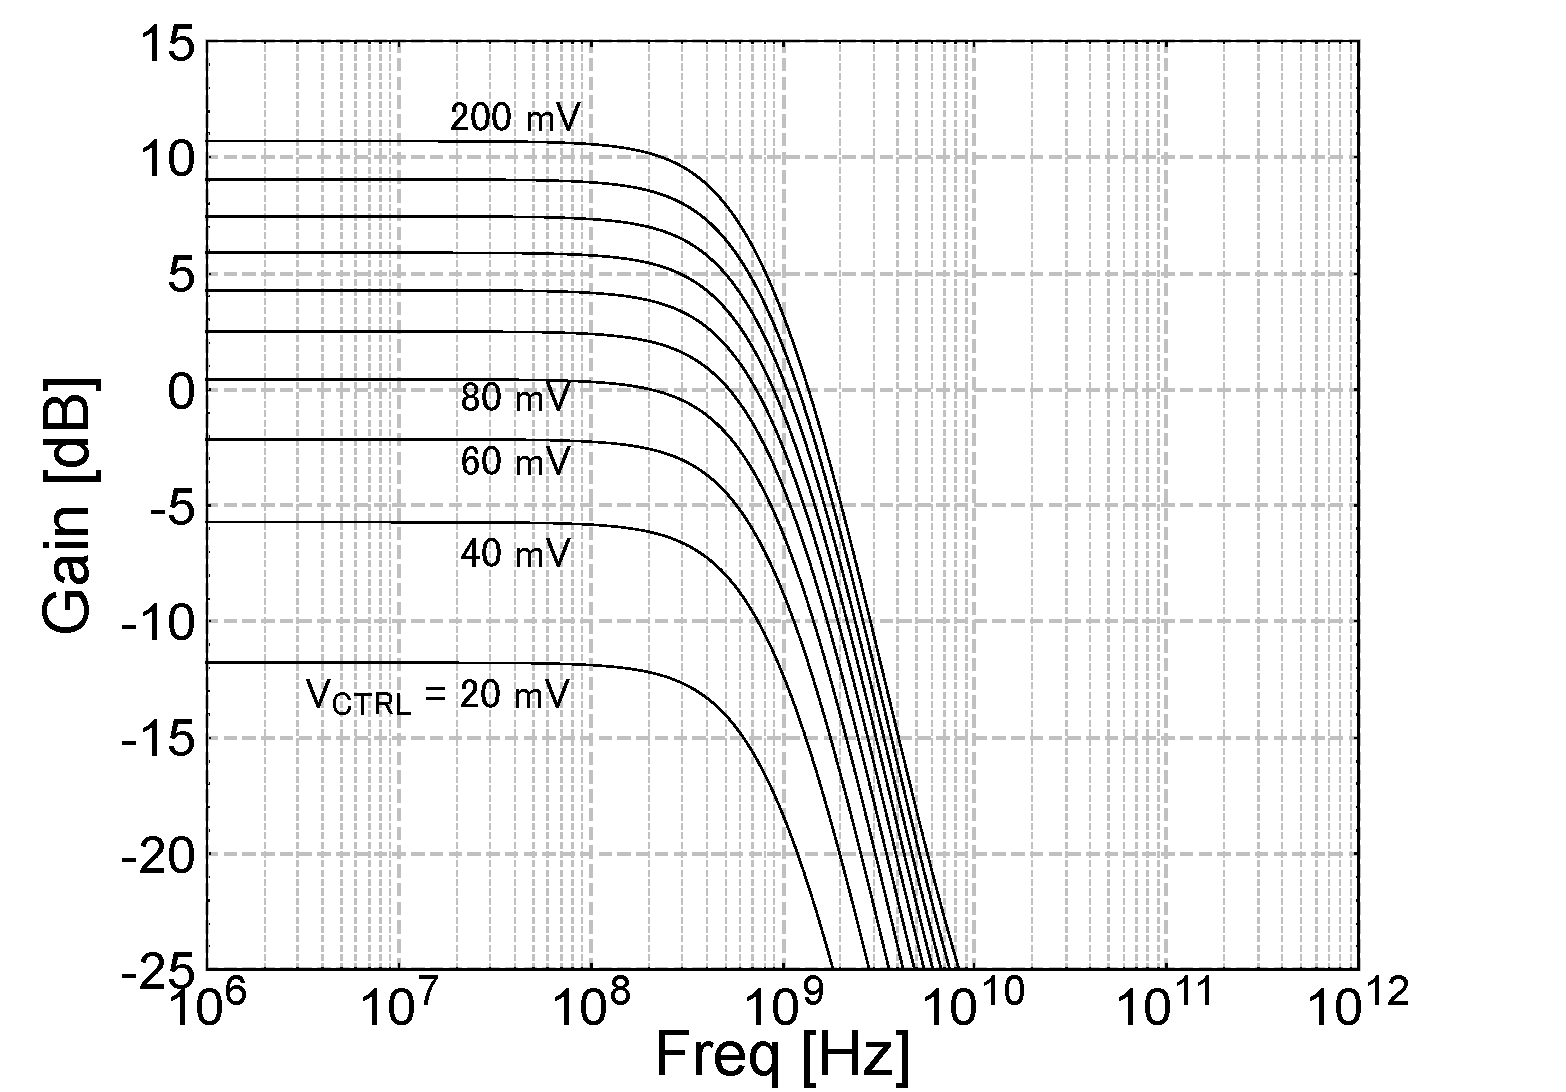
\includegraphics[width=0.99\textwidth]{figures/chapter3/folded_ac.pdf}
            \caption{折り返しカスコード型の周波数特性}
            \label{fig:3_folded_gilbert_ac}
        \end{figure}
        \clearpage
        今回の設計ではトランスコンダクタンスも揃っているので利得は同程度であるが,遮断周波数は1桁程度落ちてしまっている.本論文での目的はS/N比を向上させるために出力範囲を拡大することであるが,フォトニックリザバに用いることを想定すると周波数特性が構造的にギルバート乗算回路よりも悪化するのは避けたい.そこでPMOSFETを使用せずに信号の折り返しを行うことで出力範囲を拡大できるのではないかと考え,これを実現する回路を図\ref{fig:3_folded_mirror_gilbert}に示し,これを「カレントミラーを組み合わせた折り返し型乗算回路」とした.\par
        \begin{figure}[!b]
            \begin{center}
                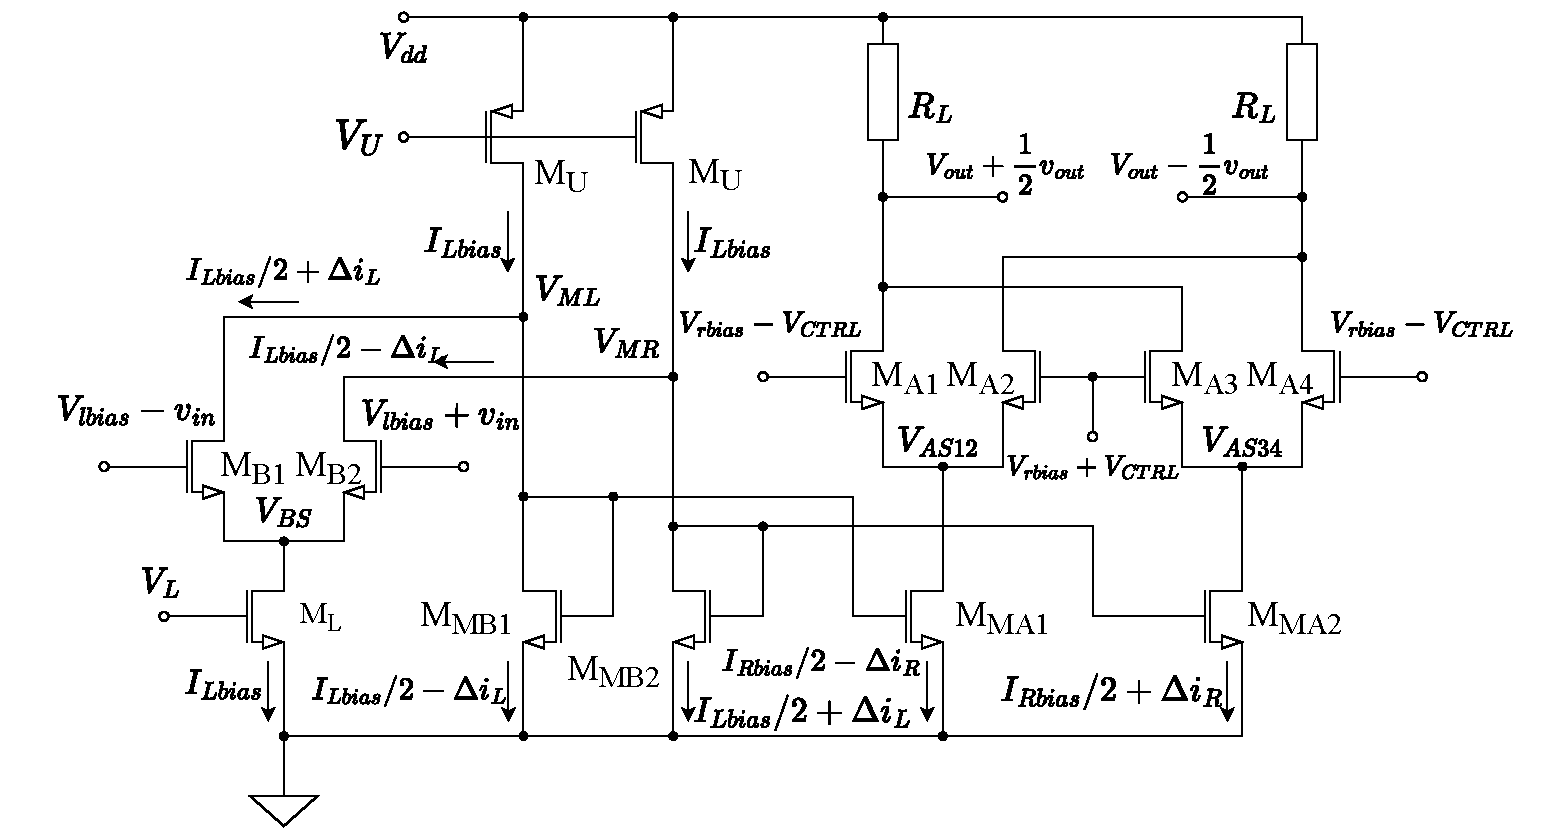
\includegraphics[width=0.99\textwidth]{figures/chapter3/NtoNFolded.pdf}
                \caption{カレントミラーを組み合わせた折り返し型乗算回路}
                \label{fig:3_folded_mirror_gilbert}
            \end{center}
        \end{figure}
        この回路では$\mathrm{M_{U},M_{L}}$をともに電流源として用いており,定電流$I_{Lbias}$を入力のMOSFETである$\mathrm{M_{B}}$とカレントミラーの参照電流を流す$M_{MB}$で分流する.これにより,入力の差動対によって$v_{in}$に比例した信号電流を符号を逆転させ$M_{MB}$に流す.カレントミラーのコピー側である$\mathrm{M_{MA}}$には$\mathrm{M_{MB}}$と$\mathrm{M_{MA}}$の形状比と$v_{in}$に比例した電流を流すことができる.これにより制御電圧を印加する$\mathrm{M_{A}}$に流れるバイアス電流を変動させる.$\mathrm{M_{A}}$はゲート接地増幅回路であり,\ref{ch:gilbert_valiable_gm}節での議論からトランスコンダクタンスは$V_{CTRL}$に比例しており,負荷抵抗$R_{L}$に流れる電流を$V_{in}$と$V_{CTRL}$に比例したものにすることができる.そして負荷抵抗によって電流を電圧に変換する.このようにしてカレントミラーと差動対で電流を分流することで折り返しカスコード型の様に信号を伝達することができるのではないかと予測し,図\ref{fig:3_folded_mirror_gilbert}の構成を考えた.


    \section{小信号解析}
        前節では今回提案する構成によって乗算ができると考える理由を述べたが,本節では小信号解析により提案回路を用いたアナログ乗算が可能であることを示す.\par
        図\ref{fig:3_folded_mirror_gilbert}はギルバート乗算回路同様差動回路であるため差動半回路を考えることで回路全体の小信号解析を行うことができる.したがって半回路として考える部分を図\ref{fig:3_folded_mirror_gilbert_half}に示す.また,この時の小信号等価半回路を図\ref{fig:3_folded_mirror_half}に示す.
        \begin{figure}[!b]
            \centering
            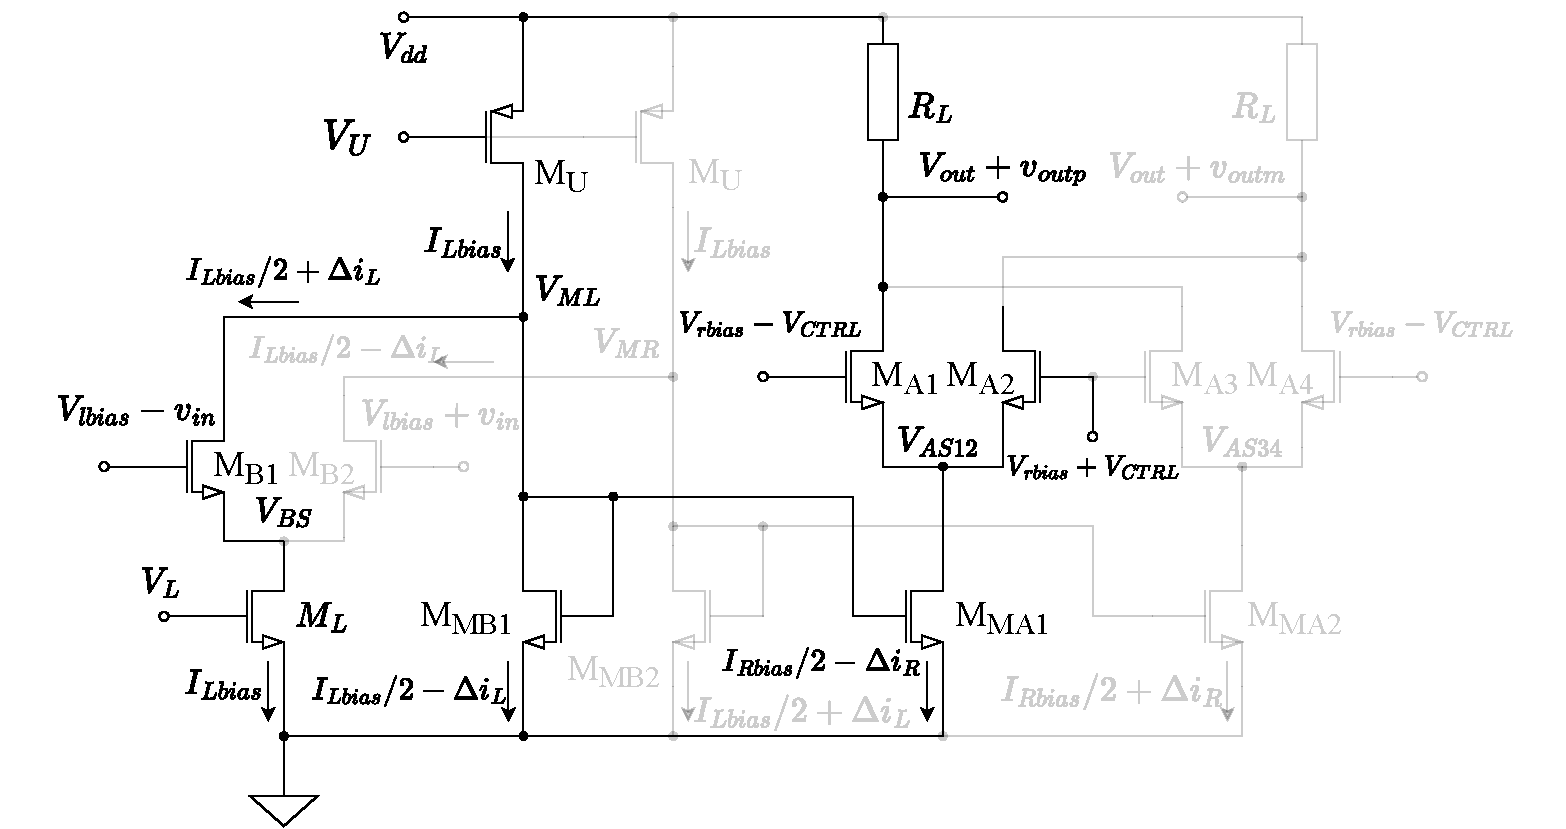
\includegraphics[width=0.99\textwidth]{figures/chapter3/NtoNFolded_half.pdf}
            \caption{カレントミラーを組み合わせた折り返し型アナログ乗算回路の半回路として考える部分}
            \label{fig:3_folded_mirror_gilbert_half}
        \end{figure}
        \begin{figure}[!b]
            \centering
            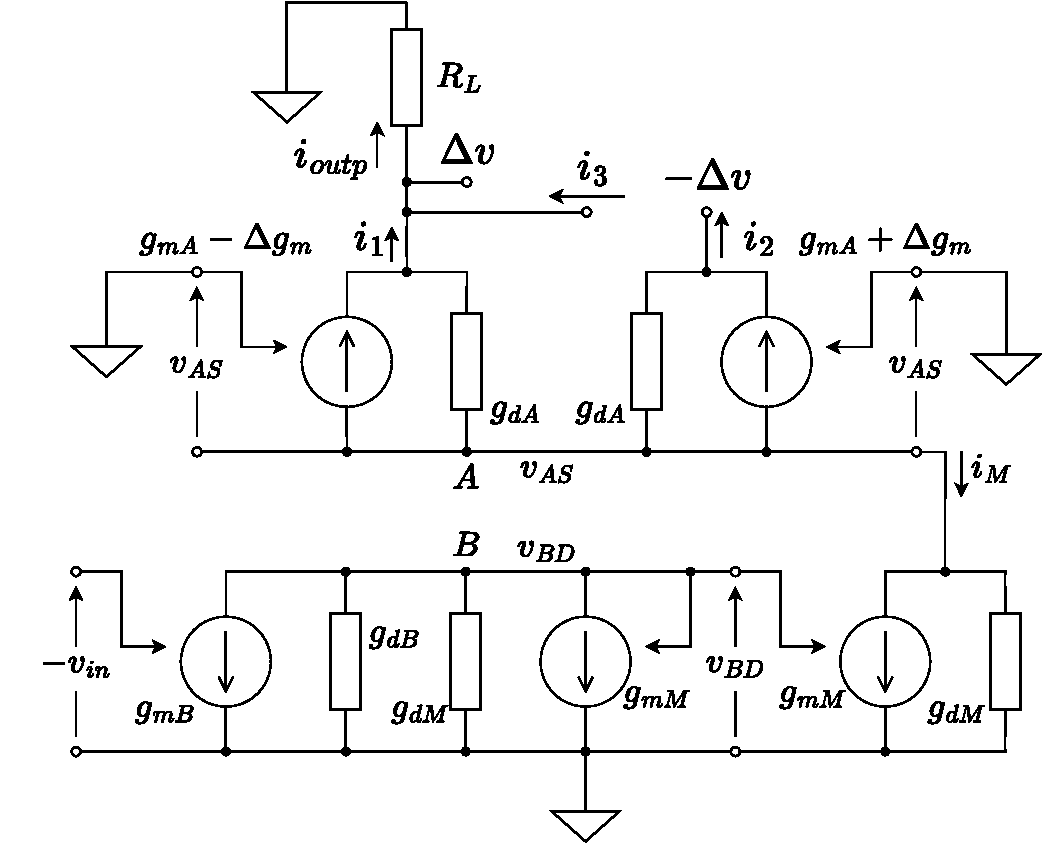
\includegraphics[width=0.99\textwidth]{figures/chapter3/NtoNHalfDiffEqual.pdf}
            \caption{カレントミラーを組み合わせた折り返し型アナログ乗算回路の小信号半回路}
            \label{fig:3_folded_mirror_half}
        \end{figure}
        \clearpage
        ここで$g_{mB},g_{mMB},g_{mMA},g_{mA}$はそれぞれ$\mathrm{M_{B},M_{MB},M_{MA},M_{A}}$のトランスコンダクタンスであり,$g_{dB},g_{dMB},g_{dMA},g_{dA}$は$\mathrm{M_{B},M_{MB},M_{MA},M_{A}}$のドレインソース間抵抗である.また$R_{L}$は負荷抵抗であり,$v_{AS},v_{BD}$はそれぞれ接点A,Bの電位とする.この時,接点BにKCLを用いると$v_{BD}$は
        \begin{align}
            0&=g_{mB}(-v_{in})+(g_{dB}+g_{dMB})v_{BD}+g_{mMB}v_{BD}     \notag\\
            v_{BD}&=\frac{g_{mB}}{ g_{mMB}+g_{dMA}+g_{dMB} }v_{in}      \notag
        \end{align}
        と表せる.ここで,$g_{mB}>>g_{dMA},g_{dMB}$を仮定すると
        \begin{align}
            v_{BD}\approx \frac{g_{mB}}{g_{mMB}}v_{in}      \label{eq:3_vbd}
        \end{align}
        と近似することができる.次に$i_{A1},i_{A2}$はそれぞれ
        \begin{align}
            i_{A1}&=(g_{mA}-\Delta g_{m})(-v_{AS})+g_{dA}(v_{outp}-v_{AS})      \label{eq:3_ia1}\\
            i_{A2}&=(g_{mA}+\Delta g_{m})(-v_{AS})+g_{dA}(v_{outm}-v_{AS})      \label{eq:3_ia2}   
        \end{align}
        であることを用いると,接点AについてのKCLを考えることで$v_{AS}$は
        \begin{align*}
            g_{mMA}v_{BD}+g_{dMA}v_{AS}&=i_{A1}+i_{A2}   \\
            &=(g_{mA}-\Delta g_{m})(-v_{AS})+g_{dA}(v_{outp}-v_{AS})    \\
            &\quad\quad\quad\quad +(g_{mA}+\Delta g_{m})(-v_{AS})+g_{dA}(v_{outm}-v_{AS})       \\
            &=-2g_{mA}v_{AS}-2g_{dA}v_{AS}  \\
            v_{AS} &= -\frac{ g_{mMA} }{ 2g_{mA}+2g_{dA}+g_{dMA} }v_{BD}
        \end{align*}
        と計算できる.さらに$g_{mMA}>>2g_{dA},g_{dMA}$を仮定すると
        \begin{align}
            V_{AS} \approx -\frac{g_{mMA}}{2g_{mA}} v_{BD}      \label{eq:3_vas}
        \end{align}
        の近似ができる.ここで図\ref{fig:3_folded_mirror_half}が差動回路であることに注意すると,\mbox{$i_{A3}=-i_{A2}$} \mbox{$v_{outp}=-v_{outm}$}の関係が成り立つので
        \begin{align}
            i_{outp}&=i_{A1}+i_{A3}     \notag\\
            &=i_{A1}-i_{A2}     \notag\\
            &=2\Delta g_{m}v_{AS}+2g_{dA}v_{outp}     \label{eq:3_ioutp}
        \end{align}
        と$v_{outp}$を用いて$i_{outp}$を表すことができた.接点OについてのKVLを考えると
        \begin{align}
            v_{outp}&=0-R_{L}i_{outp}       \notag\\
            &=-R_{L}\left( 2\Delta g_{m}v_{AS}+2g_{dA}v_{outp}  \right)       \notag\\
            &=-\frac{ 2R_{L} }{ 1+2R_{L}g_{dA} } \cdot \Delta g_{m}v_{AS}       \label{eq:3_voutp}    
        \end{align}
        であるので,出力電圧$v_{out}$を$v_{out}:=v_{outp}-v_{outm}$とすれば,$v_{outp}=-v_{outm}$であることに留意すると
        \begin{align*}
            v_{out}&=2v_{outp}  \\
            &=-\frac{ 4R_{L} }{ 1+2R_{L}g_{dA} } \cdot \Delta g_{m}v_{AS}
        \end{align*}
        と計算できる.ここで式(\ref{eq:3_vbd}),(\ref{eq:3_vas})を代入すると
        \begin{align*}
            v_{out}=\frac{ g_{mB} }{ g_{mA} }\cdot\frac{ g_{mMA} }{ g_{mMB} }\cdot\frac{ 2R_{L} }{ 1+2R_{L} g_{dA}}\cdot\Delta g_{m}v_{in}
        \end{align*}
        である.さらに\ref{ch:gilbert_valiable_gm}の結論を用いれば,$\mathrm{M_{A}}$のトランスコンダクタンス係数を$K$としたとき$\Delta g_{m}=2KV_{CTRL}$なので
        \begin{align}
            v_{out}=\frac{ g_{mB} }{ g_{mA} }\cdot\frac{ g_{mMA} }{ g_{mMB} }\cdot\frac{ 4KR_{L} }{ 1+2R_{L} g_{dA}}\cdot V_{CTRL}\cdot v_{in}      \label{eq:3_vout}
        \end{align}
        と計算することができた.したがってカレントミラーを組み合わせた折り返し型乗算回路は入力電圧$v_{in}$と制御電圧$V_{CTRL}$に比例した出力を得ることができる.特にカレントミラーの形状比が同一である場合,$g_{mMA}=g_{mMB}$となるため,ギルバート乗算回路の出力と一致することが分かる.


    \section{出力範囲}
        次に,\ref{ch:2_range}と同様の方法で出力範囲を求めギルバート乗算回路と比較を行う.まず,適切に動作する条件をすべてのMOSFETが飽和領域で動作することするための式(\ref{eq:2_binding_conditions})を再掲すると
        \begin{subequations}
            \begin{empheq}[left={\empheqlbrace}]{align*}
                &V_{GS}-V_{th}<V_{DS}          \\
                &V_{th}<V_{GS}              
            \end{empheq}
        \end{subequations}
        であった.これを図\ref{fig:3_folded_mirror_gilbert}の各MOSFETに適用すると
        \begin{subequations}
            \begin{empheq}[left={M_{A}:\empheqlbrace}]{align}
                &V_{rbias}+V_{CTRL}-V_{AS}-V_{th}<V_{out}-\frac{1}{2}v_{out}-V_{AS}        \\
                &V_{th}<V_{rbias}-V_{CTRL}-V_{AS}
            \end{empheq}        \label{eq:3_ma_binding}
        \end{subequations}
        \begin{subequations}
            \begin{empheq}[left={M_{MA}:\empheqlbrace}]{align}
                &V_{M}-V_{th}<V_{AS}        \\
                &V_{th}<V_{dd}-V_{U}
            \end{empheq}        \label{eq:3_mma_binding}
        \end{subequations}
        \begin{subequations}
            \begin{empheq}[left={M_{U}:\empheqlbrace}]{align}
                &V_{dd}+v_{in}-V_{BS}-V_{th}<V_{dd}-V_{BS}      \\
                &V_{th}<V_{dd}-V_{U}
            \end{empheq}        \label{eq:3_mu_binding}
        \end{subequations}
        \begin{subequations}
            \begin{empheq}[left={M_{B}:\empheqlbrace}]{align}
                &V_{lbias}+v_{in}-V_{BS}-V_{th}<V_{M}-V_{BS}        \\
                &V_{th}<V_{lbias}-v_{in}-V_{BS}
            \end{empheq}        \label{eq:3_mb_binding}
        \end{subequations}
        \begin{subequations}
            \begin{empheq}[left={M_{L}:s\empheqlbrace}]{align}
                &V_{L}-V_{th}<V_{BS}        \\
                &V_{th}<V_{L}
            \end{empheq}        \label{eq:3_ml_binding}
        \end{subequations}
        という5つの不等式が得られる.ただし,$\mathrm{M_{MA}}$に関してはダイオード接続になっているので常に飽和領域で動作する.まず$\mathrm{M_{L}}$について,式(\ref{eq:3_ml_binding}b)の両辺に$-V_{th}$を加えると
        \begin{align*}
            0<V_{L}-V_{th}
        \end{align*}
        となる.これと式(\ref{eq:3_ml_binding}a)と合わせると
        \begin{align}
            0<V_{BS}    \label{eq:3_vbs_range}
        \end{align}
        を得る.同様に$\mathrm{M_{A},M_{B},M_{U}}$についてもa式とb式をまとめると
        \begin{align}
            \mathrm{M_{A}}\;:\;&V_{AS}<V_{out}-\frac{1}{2}v_{out}-2V_{CTRL}        \label{eq:3_vas_upper}\\
            \mathrm{M_{B}}\;:\;&V_{BS}+2v_{in}<V_{M}                               \label{eq:3_vm_lower}\\
            \mathrm{M_{U}}\;:\;&V_{M}<V_{dd}                                       \label{eq:3_vm_upper}
        \end{align}
        と表すことができる.式(\ref{eq:3_vm_upper})に関しては,$V_{m}$が電源電圧内であれば飽和領域で動作するということなので今回は考慮する必要はない.次に式(\ref{eq:3_vas_upper})の両辺に$-V_{th}$を加えることで式(\ref{eq:3_mma_binding}a)の左辺と等しくなることに注意すると,式(\ref{eq:3_vm_lower})より
        \begin{align}
            V_{BS}+2v_{in}&<V_{out}-\frac{1}{2}v_{out}-2V_{CTRL}-V_{th}         \notag\\
            V_{BS}+2v_{in}+2V_{CTRL}+V_{th}&<V_{out}-\frac{1}{2}v_{out}         \notag\\
            \frac{1}{2}v_{out}&<V_{out}-(V_{BS}+2v_{in}+2V_{CTRL}-V_{th})        \label{eq:3_vout_lower}
        \end{align}
        を得る.また,出力電圧は電源電圧にも制限を受けるため
        \begin{align}
            V_{out}+\frac{1}{2}&<V_{dd}                                          \notag\\
            \frac{1}{2}v_{out}&<V_{dd}-V_{out}                                  \label{eq:3_vout_upper}
        \end{align}
        が必要となる.式(\ref{eq:3_vout_lower}),(\ref{eq:3_vout_upper})の辺々を足し合わせると
        \begin{align}
            v_{out}&<V_{dd}-(V_{BS}+2v_{in}+2V_{CTRL}-V_{th})                  \label{eq:3_vout_range}
        \end{align}
        と求められた.これはギルバート乗算回路の出力範囲,式(\ref{ch:2_range})と比較すると$V_{th}$だけ大きくなっていることが分かる.この出力振幅の拡大はカレントミラーによって生じており,参照側はドレインとゲートを短絡しているがコピー側では飽和領域で動作する条件からドレイン電位を参照側よりもしきい電圧$V_{th}$分下げられることに起因する.つまりカレントミラーを多数接続することでさらに$\mathrm{M_{A}}$のソース電位を下げられる可能性があるが,カレントミラーのドレインソース間電圧が小さくなるとドレイン電流が小さくなることが考えられる.


    \section{シミュレーションによる確認}
        
        出力範囲が理論上はカレントミラーの閾電圧$V_{th}$分広げられることを前節で示すことができたが,本節では$\mathrm{ROHM\;0.18\;\mu m\;Process}$においてギルバート乗算回路と比較しカレントミラーを組み合わせた折り返し型乗算回路の出力範囲が広がっていることをシミュレーションによって確認する.今回は入力電圧と制御電圧を共に$0.2\;\mathrm{V}$として設計を行う.また,\\$\mathrm{ROHM\;0.18\;\mu m\;Process}$ではトリプルウェル構造を作ることができるので,各MOSFETのバルク端子は各々のソースと短絡させた.これはしきい電圧を小さくし,設計を容易にするためである.\par
        大まかな方針として高速化をするために直流で動作する部分を除きチャネル長を最小寸法である$0.18\;\mu m$を用いることとした.まずはしきい電圧を推定するためにドレイン電流($I_{D}$)-ゲートソース間電圧($V_{GS}$)特性を調べた.ただし,ここの時のチャネル幅は$1\;\mu m$とした.また,トランスコンダクタンスは式(\ref{eq:2_gm})を再掲すると
        \begin{align*}
            g_{m}=\frac{\partial I_{D}}{\partial V_{GS}}=K(V_{GS}-V_{th})
        \end{align*}
        であった.これは$V_{GS}$に関する1次式であり,最小二乗法による近似が容易である.そのためこのトランスコンダクタンスに近似した1次関数からしきい電圧を推定した.この時のNMOSFETの$I_{D}-V_{GS}$特性,トランスコンダクタンス$g_{m}-V_{GS}$特性とその近似直線を図\ref{fig:3_vth_est}に示す.
        \begin{figure}[!b]
            \centering
            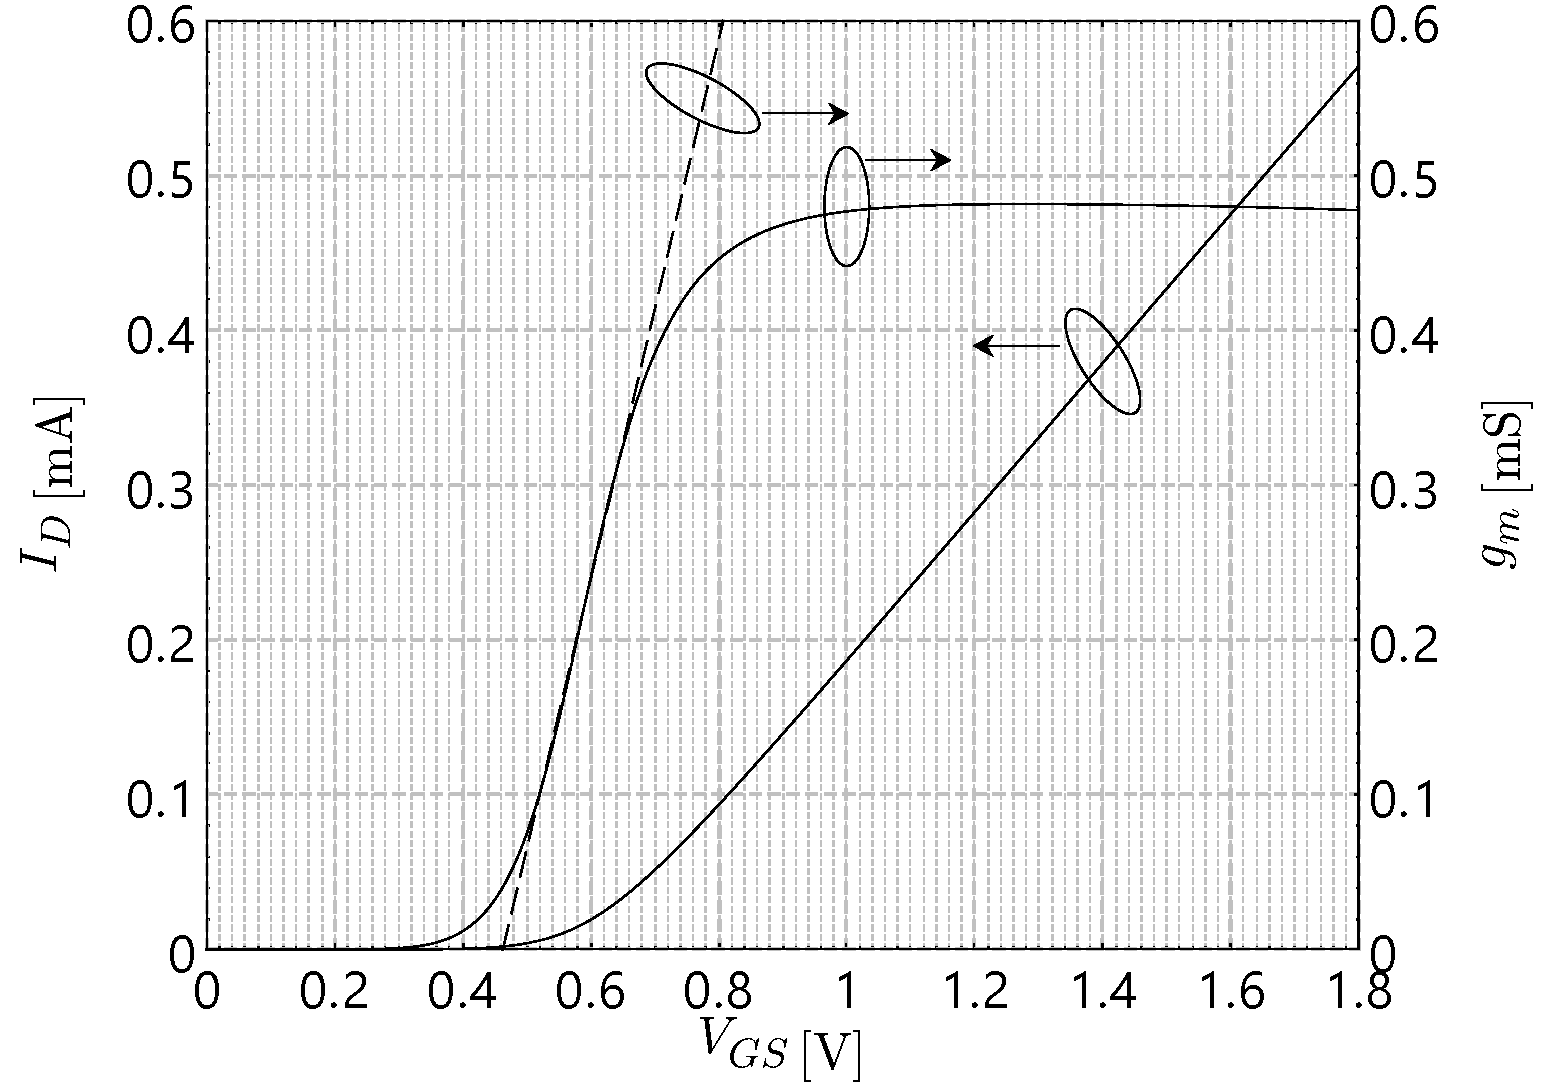
\includegraphics[width=0.99\textwidth]{figures/chapter3/id_vgs.pdf}
            \caption{$\mathrm{ROHM\;0.18\;\mu m\;Process}$における$\mathrm{(L,W)}=(0.18\;\mathrm{\mu m},1\;\mathrm{\mu m})$の時の$I_{D}-V_{GS}$,$g_{m}-V_{GS}$特性}
            \label{fig:3_vth_est}
        \end{figure}
        ただし,最小二乗法による線形近似はトランスコンダクタンスが直線的に変化していると思われる$0.5\;\mathrm{V}$から$0.65\;\mathrm{V}$の間で行った.この時の傾きは約$1.74\;\mathrm{mS/V}$,しきい電圧は約$0.46\;\mathrm{V}$であった.次に直流電位を定める.図\ref{fig:2_gilbert}において,$\mathrm{V_{S}}$の電位を$0.1\;\mathrm{V}$と定めた.これは$\mathrm{M_{C}}$は直流的に動作するため,理想的には周波数特性に影響せず,トランジスタサイズを大きくすることができるので低い電圧で動作させることとした.$\mathrm{M_{A},M_{B}}$の入力に与える直流バイアスに関しては飽和領域で使用するために自ずと決まる.$\mathrm{M_{B}}$に関して,ゲート電位は入力電圧分増減するので
        \begin{align*}
            \left( V_{B}-v_{in} \right) -V_{S} &> V_{th}  \\
            V_{B} &> 0.76
        \end{align*}
        という直流バイアスの下限が決まる.従って今回は$V_{B}=0.76\;\mathrm{V}$とした.$V_{AB}$についても,$\mathrm{M_{B}}$が飽和で動作する条件より
        \begin{align*}
            \left( V_{B}+v_{in} \right) - V_{S} -V_{th} &< V_{AB} - V_{S}   \\
            0.5 &< V_{AB}  
        \end{align*}
        と下限が定まる.$\mathrm{M_{A}}$についても同様に直流バイアスは
        \begin{align*}
            \left( V_{A}-v_{CTRL} \right) -V_{AB} &> V_{th}  \\
            V_{A} &> 1.16
        \end{align*}
        と条件が決まり,$V_{A}=1.16\;\mathrm{V}$とした.$V_{out}$の下限は
        \begin{align*}
            \left( V_{A}+v_{CTRL} \right) - V_{AB} -V_{th} &< V_{out} - \frac{1}{2}v_{out} - V_{AB}   \\
            0.9 &< V_{out} - \frac{1}{2}v_{out}
        \end{align*}
        と分かり,$V_{out}-\frac{1}{2}v_{out}=0.9\;\mathrm{V}$とした.直流電流についてはとりあえず$1\;\mathrm{mA}$とした.これはドレインソース間電圧が$0.4\;\mathrm{V}$程度でも十分流せる電流だと考え,この値とした.出力端子の直流電位は$\mathrm{M_{A}}$のドレイン端子の下限$0.9\;\mathrm{V}$と電源電圧$1.8\;\mathrm{V}$の中心である$1.35\;\mathrm{V}$になるよう,無入力状態では負荷抵抗にドレイン電流の半分が流れることを考慮し,$R_{L}=900\;\mathrm{\Omega}$とした.この直流バイアスを満たすようなトランジスタサイズを表\ref{table:3_prev_com_param}に示す.\par
        \begin{table}[!b]
                \centering
                \caption{出力範囲を比較するギルバート乗算回路}
                \label{table:3_prev_com_param}
                \begin{tabular}{c|c|r}
                    \hline
                    \multicolumn{2}{c}{Gilbert}   & \multicolumn{1}{c}{Value}     \\
                    \hline\hline
                    &   Channel Length   &   0.18 $\mathrm{\mu m}$   \\
                    \cline{2-3}
                    $\mathrm{M_{A}}$   &   Channel Width   &   4.26 $\mathrm{\mu m}$   \\
                    \cline{2-3}
                        &   Multifinger   & 2    \\
                    \hline
                    &   Channel Length   &   0.18 $\mathrm{\mu m}$   \\
                    \cline{2-3}
                    $\mathrm{M_{B}}$   &   Channel Width   &   4.26 $\mathrm{\mu m}$   \\
                    \cline{2-3}
                        &   Multifinger   & 4    \\
                    \hline
                    &   Channel Length   &   0.54 $\mathrm{\mu m}$   \\
                    \cline{2-3}
                    $\mathrm{M_{C}}$   &   Channel Width   &   17 $\mathrm{\mu m}$   \\
                    \cline{2-3}
                        &   Multifinger   & 10    \\
                    \hline
                    \multicolumn{2}{c|}{$\mathrm{V_{dd}}$} &   $1.8\;\mathrm{V}$   \\
                    \hline
                    \multicolumn{2}{c|}{$\mathrm{V_{A}}$} &   $1.16\;\mathrm{V}$   \\
                    \hline
                    \multicolumn{2}{c|}{$\mathrm{V_{B}}$} &   $0.76\;\mathrm{V}$   \\
                    \hline
                    \multicolumn{2}{c|}{$\mathrm{V_{C}}$} &   $0.6;\mathrm{V}$   \\
                    \hline
                    \multicolumn{2}{c|}{$\mathrm{R_{L}}$} &   $900\;\mathrm{\Omega}$   \\
                    \hline
                \end{tabular}
        \end{table}
        次にカレントミラーを組み合わせた折り返し型乗算回路の素子値の設計を行う.まず,$\mathrm{M_{B},M_{L}}$についてはギルバート乗算回路と同様の素子値,直流電位とした.次に$\mathrm{M_{MB}}$の素子値を$\mathrm{M_{B}}$と同様にすると,$\mathrm{M_{B}}$のゲートソース間電圧と$\mathrm{M_{MB}}$のドレインソース間電圧が等しくなった時に同じ大きさの電流が流れる.つまり,$\mathrm{M_{B}}$のゲート端子の直流電位$V_{lbias}$から$\mathrm{M_{B}}$のソース電位$V_{BS}$を引いた$0.66\;\mathrm{V}$が$V_{M}$の直流電位となる.このとき,入力$v_{in}$を$-0.2\;\mathrm{V}$から$0.2\;\mathrm{V}$まで掃引すると,$V_{M}$の最大値はおよそ$0.76\;\mathrm{V}$であった.従って,電流源$\mathrm{M_{U}}$はこの直流バイアスで$1\;\mathrm{mA}$の流すことができる形状とした.したがって,$\mathrm{M_{MA}}$が飽和領域で動作するためには
        \begin{align*}
            0.76-V_{th} &< V_{AS}      \\
            0.3 &< V_{AS}
        \end{align*}
        が必要となる.同様にして$\mathrm{M_{A}}$については
        \begin{align*}
            \left( V_{rbias}-V_{CTRL} \right) -V_{AS} &> V_{th}     \\
            V_{rbias} &> 0.96
        \end{align*}
        と分かった.さらに出力電位に関しては
        \begin{align*}
            \left( V_{rbias}+V_{CTRL} \right) - V_{AS} - V_{th} &< V_{out} - v_{AS} \\
            0.7 &< V_{out} - \frac{1}{2}v_{out}
        \end{align*}
        であるので,出力範囲の下限は$0.7\;\mathrm{V}$とすることとした.$\mathrm{M_{A}}$のサイズを$\mathrm{M_{B}}$のサイズと同様にし並列数を半分にすると$\mathrm{M_{MA}}$に流れる電流は$\mathrm{M_{B}}$と等しくなる.したがって,負荷抵抗の値を無信号時に出力範囲の中間になるように決めると$1.1\;\mathrm{k\Omega}$となる.$\mathrm{M_{MA}}$の形状は$\mathrm{M_{MB}}$と同様にした.以上の素子値でも乗算は可能だが,増幅率がすこし足りなかったので素子値を調整した.最終的なカレントミラーを組み合わせた折り返し型乗算回路の素子値を表\ref{table:3_folded_mirror_com_param}に示す.
        \begin{table}[!b]
            \centering
            \caption{出力範囲を比較するカレントミラーを組み合わせた折り返し型乗算回路}
            \label{table:3_folded_mirror_com_param}
            \begin{tabular}{c|c|r}
                    \hline
                    \multicolumn{2}{c}{Gilbert}   & \multicolumn{1}{c}{Value}     \\
                    \hline\hline
                    &   Channel Length   &   0.18 $\mathrm{\mu m}$   \\
                    \cline{2-3}
                    $\mathrm{M_{A}}$   &   Channel Width   &   4.26 $\mathrm{\mu m}$   \\
                    \cline{2-3}
                        &   Multifinger   & 4    \\
                    \hline
                    &   Channel Length   &   0.18 $\mathrm{\mu m}$   \\
                    \cline{2-3}
                    $\mathrm{M_{B}}$   &   Channel Width   &   4.26 $\mathrm{\mu m}$   \\
                    \cline{2-3}
                        &   Multifinger   & 4    \\
                    \hline
                    &   Channel Length   &   0.18 $\mathrm{\mu m}$   \\
                    \cline{2-3}
                    $\mathrm{M_{MA}}$   &   Channel Width   &   4.26 $\mathrm{\mu m}$   \\
                    \cline{2-3}
                        &   Multifinger   & 8    \\
                    \hline
                    &   Channel Length   &   0.18 $\mathrm{\mu m}$   \\
                    \cline{2-3}
                    $\mathrm{M_{MB}}$   &   Channel Width   &   4.26 $\mathrm{\mu m}$   \\
                    \cline{2-3}
                        &   Multifinger   & 4    \\
                    \hline
                    &   Channel Length   &   0.72 $\mathrm{\mu m}$   \\
                    \cline{2-3}
                    $\mathrm{M_{U}}$   &   Channel Width   &   5.26u $\mathrm{\mu m}$   \\
                    \cline{2-3}
                        &   Multifinger   & 8    \\
                    \hline
                    &   Channel Length   &   0.54 $\mathrm{\mu m}$   \\
                    \cline{2-3}
                    $\mathrm{M_{L}}$   &   Channel Width   &   17 $\mathrm{\mu m}$   \\
                    \cline{2-3}
                        &   Multifinger   & 10    \\
                    \hline
                    \multicolumn{2}{c|}{$\mathrm{V_{dd}}$} &   $1.8\;\mathrm{V}$   \\
                    \hline
                    \multicolumn{2}{c|}{$\mathrm{V_{rbias}}$} &   $0.96\;\mathrm{V}$   \\
                    \hline
                    \multicolumn{2}{c|}{$\mathrm{V_{lbias}}$} &   $0.76\;\mathrm{V}$   \\
                    \hline
                    \multicolumn{2}{c|}{$\mathrm{V_{U}}$} &   $0.5\;\mathrm{V}$   \\
                    \hline
                    \multicolumn{2}{c|}{$\mathrm{V_{L}}$} &   $0.6\;\mathrm{V}$   \\
                    \hline
                    \multicolumn{2}{c|}{$\mathrm{R_{L}}$} &   $1.1\;\mathrm{K \Omega}$   \\
                    \hline
            \end{tabular}
        \end{table}
        これらの素子値においての直流解析結果を図\ref{fig:3_previous_dc_com},\ref{fig:3_folded_mirror_dc_com}に,交流解析結果を図\ref{fig:3_previous_ac_com},\ref{fig:3_folded_mirror_ac_com}に示す.
        図\ref{fig:3_previous_dc_com},\ref{fig:3_folded_mirror_dc_com}のどちらも適切に入力電圧と制御電圧に比例した電圧出力を得ることが確かめられた.また,ギルバート乗算回路では出力振幅は$\pm 0.8\mathrm{\;V}$程度であったが,カレントミラーを組み合わせた折り返し型乗算回路では$\pm 1.3\mathrm{\;V}$程度の振幅を得ることができている.ギルバート乗算回路については,式(\ref{eq:2_range_out})に今回使用した値を代入すると$0.9 <v_{out}$となるため今回のシミュレーション結果はその範囲内に入っている.同様に,カレントミラーを組み合わせた折り返し型乗算回路については,式(\ref{eq:3_vout_range})に値を代入すると$1.3 < v_{out}$となる.こちらも理論式の範囲内であった.次に交流解析結果について,遮断周波数はギルバート乗算回路でおよそ$7\;\mathrm{GHz}$程度,カレントミラーを組み合わせた折り返し型乗算回路で$3\;\mathrm{GHz}$程度と劣化はしている結果となった.一つの要因としてはカレントミラーが信号の伝達にかかわっているので,ギルバート乗算回路にはないその部分が周波数特性劣化の原因になりうるということが考えられる.また,通過するMOSFETが増えたためゲートのキャパシタンス成分が増加し遮断周波数が低下したことが考えらえる.ただ,出力振幅の拡大は確認でき,周波数特性の劣化はPMOSFETを使用した折り返しカスコード型よりも抑えることができた.\clearpage
        \begin{figure}[!b]
            \centering
            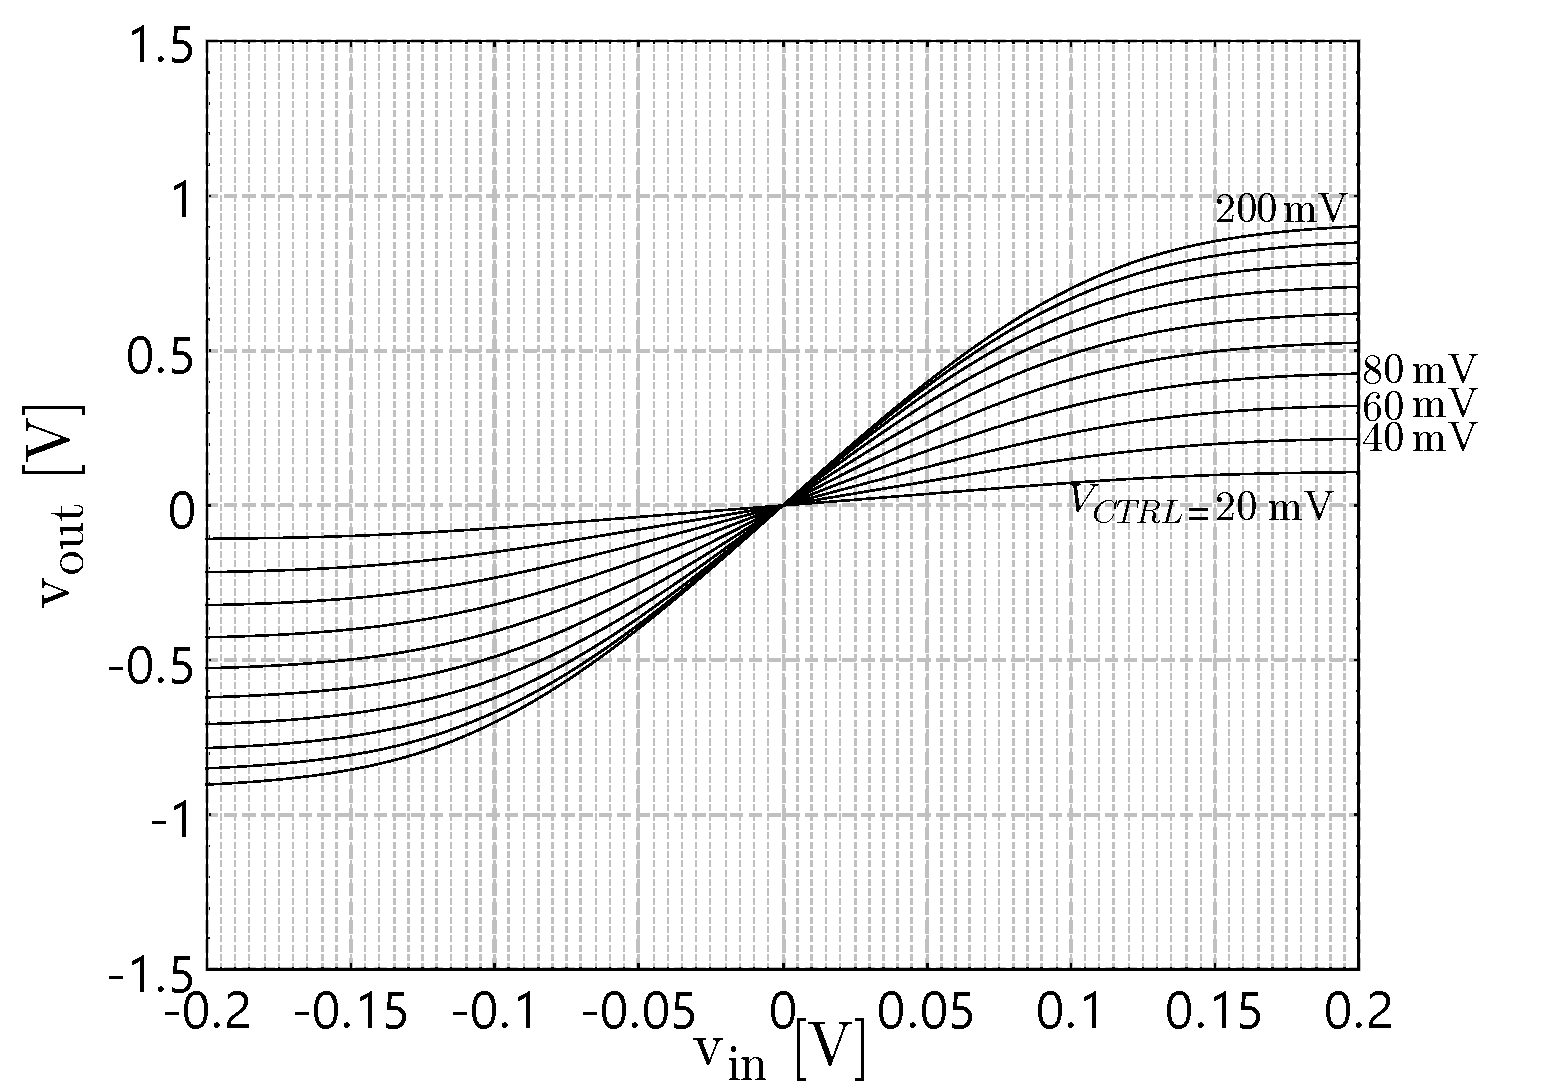
\includegraphics[width=0.9\textwidth]{figures/chapter3/previous_dc_com.pdf}
            \caption{設計したギルバート乗算回路の直流解析結果}
            \label{fig:3_previous_dc_com}
        \end{figure}
        \begin{figure}[!b]
            \centering
            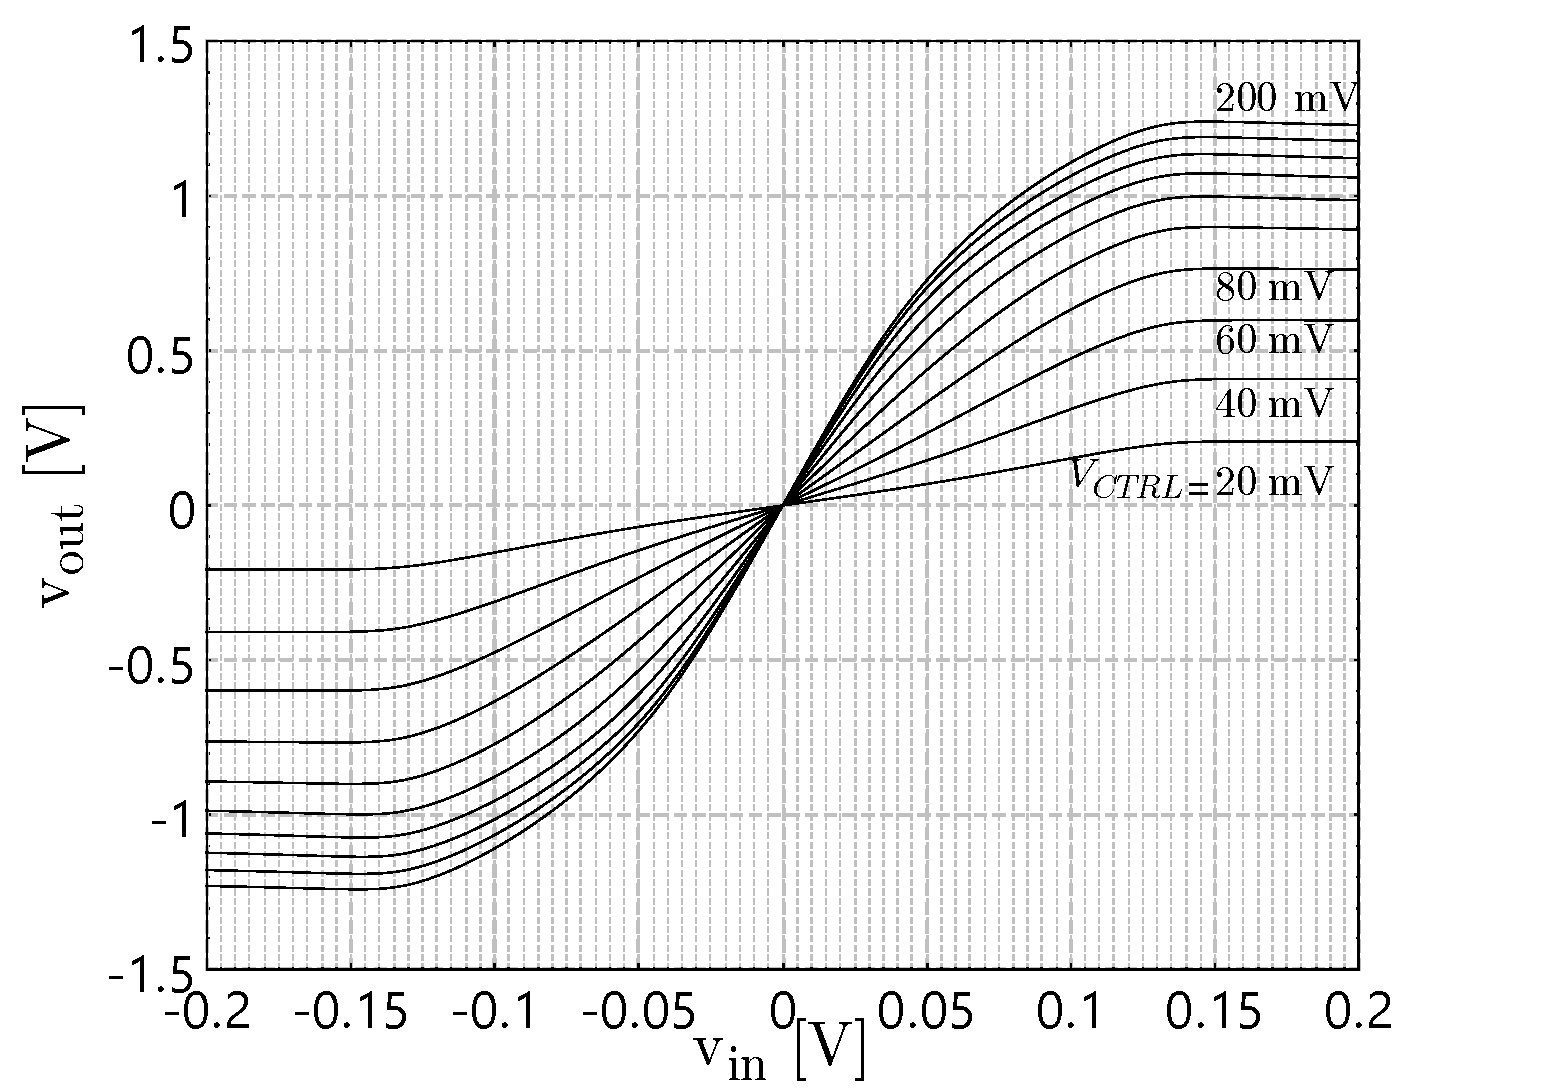
\includegraphics[width=0.9\textwidth]{figures/chapter3/folded_mirror_dc_com.pdf}
            \caption{設計した折り返しカスコード型乗算回路の直流解析結果}
            \label{fig:3_folded_mirror_dc_com}
        \end{figure}
        \begin{figure}[!b]
            \centering
            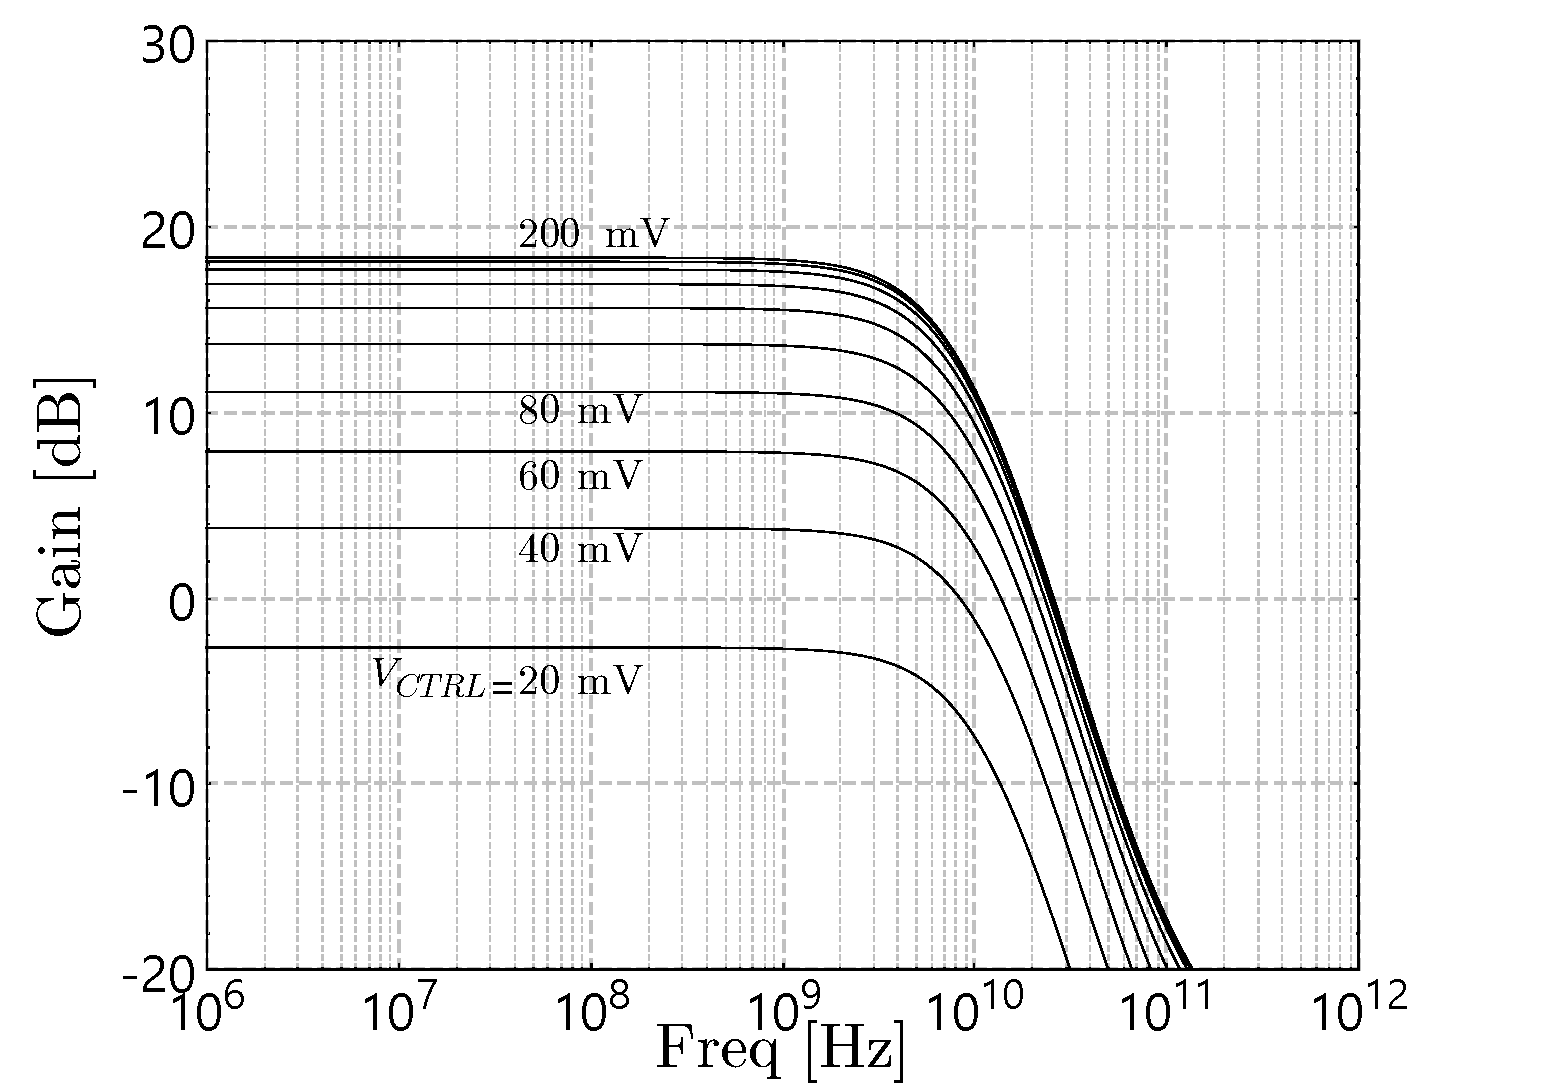
\includegraphics[width=0.95\textwidth]{figures/chapter3/previous_ac_com.pdf}
            \caption{設計したギルバート乗算回路の交流解析結果}
            \label{fig:3_previous_ac_com}
        \end{figure}
        \begin{figure}[!b]
            \centering
            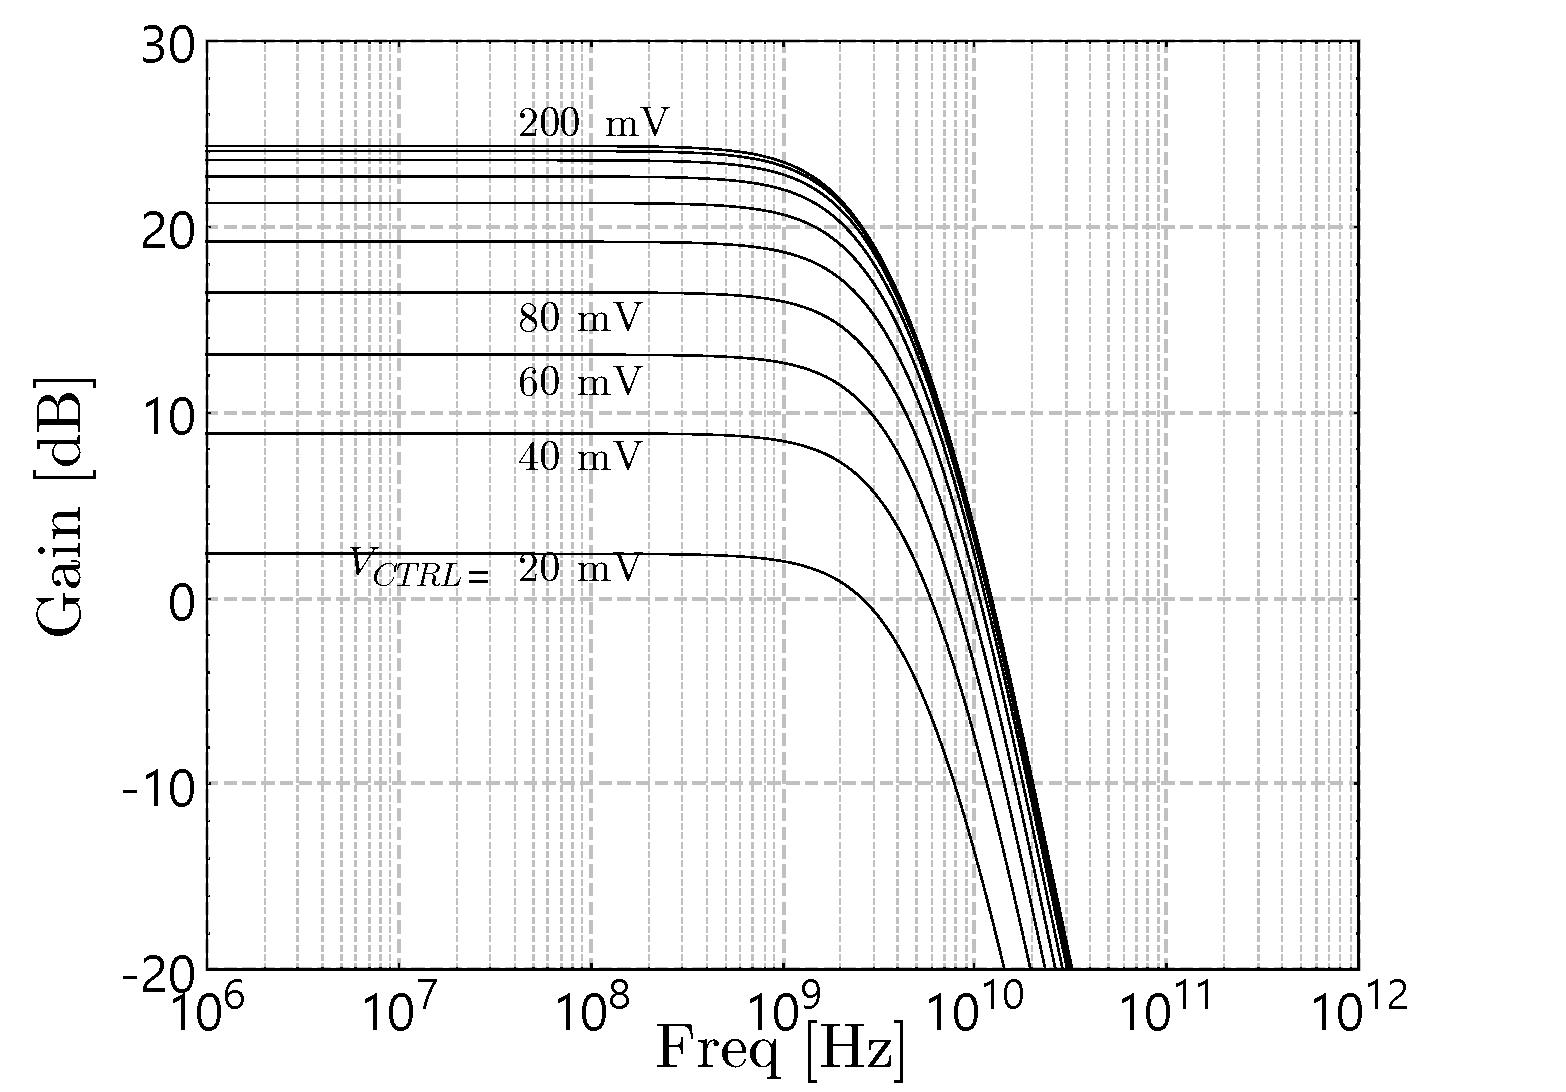
\includegraphics[width=0.95\textwidth]{figures/chapter3/folded_mirror_ac_com.pdf}
            \caption{設計したカレントミラーを組み合わせた折り返し型乗算回路の乗算回路の交流解析結果}
            \label{fig:3_folded_mirror_ac_com}
        \end{figure}

        

%    \begin{figure}[!b]
%        \centering
%        \includegraphics[width=0.99\textwidth]{figures/chapter}
%        \caption{}
%        \label{fig:3_}
%    \end{figure}

%    \begin{subequations}
%        \begin{empheq}[left={\empheqlbrace}]{align}
%        \end{empheq}        \label{eq:}
%    \end{subequations}
